\section{Máquinas de Turing}
El modelo más básico de una máquina de turing  consiste en un control finito, una cinta infinita dividida en celdas y una cabeza de lectura. Cada celda de la cinta puede contener un único símbolo del alfabeto finito de la cinta.

Inicialmente, la cinta contiene una cadena de símbolos de entrada, seguida de un símbolo especial llamado blanco. La cabeza de lectura se coloca sobre el primer símbolo de la cadena de entrada. La máquina de Turing puede leer y escribir símbolos en la cinta o mover la cabeza de lectura a la izquierda o a la derecha.
\begin{figure}[H]
  \begin{center}
    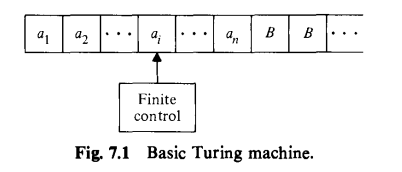
\includegraphics[scale=0.75]{imagenes/mt.png}
  \end{center}
\end{figure}
Formalmente, definimos la máquina de Turing (MT) \(M\) como una tupla:
\[
  M = \langle Q, \Sigma, \Gamma, \delta, q_0, B, F \rangle
\]

Donde:
\begin{itemize}
  \item \(Q\) es un conjunto finito de estados.
  \item \(\Sigma\) es un alfabeto de entrada.
  \item \(\Gamma\) es un alfabeto de cinta.
  \item \(\delta: Q\times\Gamma\to Q\times\Gamma\times\{L, R\}\) es una función de transición. Podría estar indefinido para algunos argumentos. La función indica devuele el estado al que se debe pasar, el símbolo a escribir en la posición actual de la cinta y el movimiento del cabezal (izquierda o derecha).
  \item \(q_0 \in Q\) es el estado inicial.
  \item \(B \in \Gamma\) es el símbolo blanco.
  \item \(F \subseteq Q\) es el conjunto de estados finales.
\end{itemize}

\paragraph{Configuración instantanea:} Una configuración instantánea de una MT es una tupla \(\alpha_1 q \alpha_2\) donde \(q\in Q\) y \(\alpha_1,\alpha_2\in\Gamma^*\) donde:
\begin{itemize}
  \item \(\alpha_1\) son los simbolos de la cinta a la izquierda del cabezal.
  \item \(q\) es el estado actual.
  \item \(\alpha_2\) son los símbolos de la cinta a la derecha del cabezal hasta el último símbolo distinto de \(B\).
\end{itemize}
Notemos que \(\alpha_1,\alpha_2\in\Gamma^*\), osea que pueden tener apariciones de \(B\).

Asumismos que el cabezal está escaneando el símbolo más a la derecha de \(\alpha_2\) o un blanco si \(\alpha_2=\lambda\).

\paragraph{Movimiento del cabezal:} El movimiento del cabezal se define como sigue: Sea \[X_1\dots X_{i-2}qX_{i}\dots X_n\]una configuración instantánea de una MT \(M\).

Supongamos que \(\delta(q,X_i) = (p, Y, L)\):
\begin{itemize}
  \item Si \(i -1 = n\), asumimos \(X_i = B\)
  \item Si \(i = 1\) entonces es imposible moverse a la izquierda.
  \item Si \(1 < i < n\) entonces escribimos:
        \[
          X_1\dots X_{i-1}qX_{i}\dots X_n \underset{M}{\vdash} X_1\dots X_{i-2}pX_{i-1}YX_{i+1}\dots X_n
        \]

        En caso de haya algún sufijo de \(X_{i-1}YX_{i+1}\dots X_n\) que sea completamente blanco, entonces se elimina.
\end{itemize}

Similarmente, si \(\delta(q,X_i) = (p, Y, R)\):
\[
  X_1\dots X_{i-1}qX_{i}\dots X_n \underset{M}{\vdash} X_1\dots X_{i-1}YpX_{i+1}\dots X_n
\]

Si dos configuraciónes instantáneas están relacionadas por \(\resulta{M}\), entonces decimos que la segunda es un resultado de la primera.

Si una configuración instantánea resulta de otra en un número fínito de pasos, entonces están relacionadas por el símbolo \(\resultam{M}\).

\paragraph{Lenguaje aceptado por una MT:} Definimos al lenguaje aceptado por una MT \(M=\langle Q, \Sigma, \Gamma, \delta, q_0, B, F \rangle\) como:
\[
  \mathcal{L}(M) = \{ \omega \in \Sigma^*  : q_0\omega \resultam{M} \alpha_1 p\alpha_2 \text{ con } p\in F \land \alpha_1,\alpha_2\in\Gamma^* \}
\]

Asumimos que la máquina de Turing se detiene cuando el input es aceptado. Además es posible que nunca se detenga si el input no es aceptado.

\subsection{Autómatas linealmente acotados}
Es una máquina de Turing  no deterministica que cumple con las siguientes condiciones:
\begin{enumerate}
  \item El alfabeto de entrada incluye dos símbolos especiales (\textcentoldstyle~y \textdollar) que son utilizados como topes izquierdo y derecho, respectivamente.
  \item El autómata no se mueve ni a la izquierda de \textcentoldstyle ni a la derecha de \textdollar, ni los sobreescribe.
\end{enumerate}

\subsubsection*{Máquinas de dos cintas}
Una máquina de Turing con dos o más cintas puede simularse usando la defición dada anteriormente. Para ello, definimos los estados en \(\Gamma\) como tuplas \([x_1, x_2]\) donde \(x_i\) sería el símbolo guardado en la \(i\)-ésima cinta.


\begin{teorema}
  Si \(L\) es un lenguaje dependiente del contexto, entonces existe un autómata linealmente acotado \(A\) tal que \(\mathcal{L}(A) = L\).
\end{teorema}

\begin{demo}[0.8\textwidth]
  Se construye el autómata linealmente acotado \(M\) tal que:
  \begin{enumerate}
    \item La primera cinta contiene la cadena de entrada \textcentoldstyle\(\omega\)\textdollar.
    \item La segunda cinta se utiliza para generar las formas de la derivación. En cualquie instante, esta cinta contendrá la forma sentencial \(\alpha\) que representa la derivación de la cadena de entrada. Se inicializa con el símbolo distingido \(S\).
  \end{enumerate}

  El autómata funcionará de la siguientes manera:
  \begin{enumerate}
    \item Si \(\omega=\lambda\), entonces \(M\) se detiene rechanzando la cadena de entrada.
    \item Sino:
          \begin{enumerate}
            \item Selecciona (en forma no deterministica) la posición \(i\) dentro de \(\alpha\) (la derivación que se encuentra en la cinta)
            \item Selecciona (en forma no deterministica) la producción \(\beta\to\gamma\in P\).
            \item Si \(\beta\) aparece a partir de la posición \(i\) en \(\alpha\), entonces remplaza \(\beta\) por \(\gamma\) en \(\alpha\).
            \item Si la nueva forma sentencial \(\alpha\) es tal que \(|\alpha| > |\omega|\), entonces \(M\) se detiene rechazando la cadena de entrada.
            \item Sino, comparamos \(\alpha\) con \(\omega\). Si son iguales, entonces \(M\) se detiene aceptando la cadena de entrada. Sino, se vuelve a repetir el paso 2.
          \end{enumerate}
  \end{enumerate}
\end{demo}

\subsection{Lenguajes recursivos}
Son lenguajes \(L\) sobre un alfabeto \(\Sigma\) para el cual existe una máquina de Turing que se detiene para todo \(\alpha\in\Sigma^*\) y la acepta (termina en un estado final) si \(\alpha\in L\) o la rechaza (termina en un estado no final) si \(\alpha\notin L\). En otras palabras, son los lenguajes para los cuales existe un algoritmo que permite decidir la pertenencia (o no) de toda cadena al lenguaje.

\begin{teorema}\label{teorema:recursividad}
  Todo lenguaje dependiente del contexto es recursivo
\end{teorema}

\begin{demo}[0.8\textwidth]
  Sea \(G=\langle N, \Sigma, P, S \rangle\) un gramática dependiente del contexto y \(\omega\in\Sigma^*\). Vamos a construir un grafo fínito en el cual cada nodo tiene asocida un \(\alpha\in(V_N\cup V_T)^+\) con \(|\alpha| \leq |\omega|\). Las arista representas una producción de \(G\), osea si \(\gamma_1\tau\gamma_2\) y \(\gamma_1\beta\gamma_2\) son dos nodos, entonces van a estar conectados si y solo si \(\tau\to\beta\in P\).

  Por ser \(G\) dependiente del contexto, vale \(|\tau|\leq |\beta|\), entonces \(|\gamma_1\tau\gamma_2|\leq |\gamma_1\beta\gamma_2|\). Por lo tanto, el grafo es acotado.

  En este grafo finito, es cierto que \(S\underset{G}{\deriva}\omega\) si y solo si existe un camino desde el nodo correspondiente a \(S\) hasta el nodo correspondiente a \(\omega\). Y esto último es decidible, o sea, tiene algoritmo. Por lo tanto, \(G\) es recursivo.
\end{demo}

\begin{lemma}
  Sea \(M_1, M_2, \dots\) una enumeración de un conjunto de máquinas de Turing que paran para todas las entadradas. Siempre existe un lenguaje recursivo que no es aceptado por ninguna de ellas, o sea, siempre existe un lenguaje \(L\) tal que \(L\) es recursivo y \(L\notin\mathcal{L}(M_i)\) para todo \(i\).
\end{lemma}

\begin{demo}[0.8\textwidth]
  Consideremos el lenguaje definido \( L = \{ \omega_i : \omega_i \notin \mathcal{L}(M_i)\}\), es decir \(L\) está formado por todas las cadenas que son rechazadas por alguna de las máquinas \(M_i\). Como es decidible si \(\omega_i\in L\) o no (pues simplemente corremos las \(M_i\) con entrada \(\omega\) y vemos si para en un estado no final), entonces \(L\) es recursivo.

  Supongamos ahora que este lenguaje es aceptado por alguna de las máquinas enumeradas. Sea \(M_j\), la misma. Entonces ¿que pasa si \(\omega_j\in L\)?

  Por definición de \(L\) tenemos que \(w_j\in L \iff w_j\notin \mathcal{L}(M_j) \iff w_j \notin L\). Esto es un absurdo, por lo tanto \(L\) no es aceptado por ninguna máquina \(M_1,M_2,\dots\).
\end{demo}

\begin{lemma}
  Existe un lenguaje recursivo que no es dependiente del contexto
\end{lemma}
\begin{demo}[0.8\textwidth]
  Vamos a tratar de demostrar que podemos encontrar una numeración de máquinas Turing correspondientes a cada uno de los lenguajes dependientes del contexto definidos sobre \(\{0,1\}^*\).
\end{demo}
\begin{demoPart}[0.8\textwidth]
  Estas máquinas de Turing paran en todas las entradas porque como los lenguajes son dependientes de contexto, siempre hay un algoritmo de reconomcimiento cuando el lenguaje es dependiente del contexto.

  Codifiquemos todas estas gramaticas con cadenas binarias, es decir, demos una representación binaria a cada símbolo de la gramática codificando:

  \begin{itemize}
    \item \(0 = 10\)
    \item \(1 = 100\)
    \item y al resto de los simbolos \(s_k = 10^k\)
  \end{itemize}

  Gracias a esta codificación mediante 0s y 1s, podemos enumerarlas de la siguientes manera: \(G_1,G_2,\dots\). Además, por el teorema \ref{teorema:recursividad}, existen autómatas \(M_1, M_2,\dots\) que aceptan los lenguajes generados por cada una de ellas.

  Luego, por el lema, anterior, tenemos que existe un lenguaje \(L\) recursivo que no es aceptado por ninguno de estos autómatas y no es dependiente del contexto.
\end{demoPart}
\subsection{Máquinas de Turing No Deterministicas}
\begin{teorema}
  Sea \(M\) una máquina de Turing no deterministica y \(L = \mathcal{L}(M)\). Entonces existe una máquina de Turing determinista \(M'\) que acepta el mismo lenguaje.
\end{teorema}

\begin{demo}[0.8\textwidth]
  Sea \(r\) la máxima cantidad posible de transiciones que parte de un estado cualquiera de \(M\). Numeremos, para cada estado, las transiciones que parten de él con números entre 1 y \(r\).

  Entonces toda secuencia finita de enteros entre 1 y \(r\) representa un camino en \(M\) partiendo desde el estado inicial \(q_0\). Algunas de estas secuencias no serán ejecutables por no existir alguna de sus transiciones.

  Podemos construir una máquina de turing \(M'\) de tres cintas tal que:
  \begin{itemize}
    \item La primera contiene la entrada de \(M\)
    \item La segunda, una secuencia de enteros entre 1 y \(r\) que corresponderá a una secuencia de transiciones a partir del estado inicial \(q_0\).
    \item La tercera servirá para simular la \(M\).
  \end{itemize}
  Y funcionará de la siguiente manera:
  \begin{itemize}
    \item Generamos secuencias de enteros con valroes entre 1 y \(r\) en orden creciente de longitud y alfabetico, que irán siendo escritos en la segunda cinta.
    \item Para cada secuencia:
  \end{itemize}
\end{demo}
\begin{demoPart}[0.8\textwidth]
  \begin{itemize}
    \item[]
      \begin{enumerate}
        \item Borramos el contenido de la cinta 3
        \item Copiamos el contenido de la cinta 1 en la cinta 3.
        \item Simulamos la MT en la cinta 3 ejecutando la secuencia de transiciones en la cinta 2.
        \item Aceptamos la cadena de la cinta 1 si se acepta esa cadena en la simulación que corremos en la cinta 3.
      \end{enumerate}
    \item Cuando la cadena analizada no es aceptada por \(M\), \(M'\) no parará.
  \end{itemize}
\end{demoPart}

\begin{teorema}
  Sea \(L\) el lenguaje de la gramática \(G = \langle V_N, V_T, P, S\rangle\). Entonces existe una máquina de Turing \(M\) que acepta el mismo lenguaje.
\end{teorema}

\begin{demo}[0.8\textwidth]
  Podemos construir una máquina de Turing \(M\) no deterministica de dos cintas tal que:
  \begin{itemize}
    \item la primera contiene la cadena de entrada \(\omega\)
    \item La segunda contiene la forma setencial \(\alpha\) de la derivación de la cadena de entrada. Se inicializa con el símbolo inicial de la gramática \(S\).
  \end{itemize}

  Y opera de la siguiente manera:
  \begin{enumerate}
    \item Seleccionar (en forma no-deterministica) la posición \(i\) dentro de \(\alpha\)
    \item Seleccionar de forma no-deterministica una regla de producción \(\beta \rightarrow \gamma\in P\)
    \item Si \(\beta\) aparece a partir de la posición \(i\) en \(alpha\), entonces reemplazar \(\beta\) por \(\gamma\) en \(alpha\).
    \item Comparar la nueva forma sentencial \(\alpha\) con la cadena de entrada \(\omega\). Si son iguales, entonces aceptar la cadena de entrada. Si no, volver al paso 1.
  \end{enumerate}
\end{demo}

\begin{teorema}
  Sea \(L\) el lenguaje aceptado por una máquina de Turing \(M\). Entonces existe una gramática sin restricciones \(G\) que genera el mismo lenguaje.
\end{teorema}

\begin{demo}[0.8\textwidth]
  Vamos a armar una gramática que genere dos copias de alguna representación de la cadena de entrada y que luego simule la operación de la maquina de Turing sobre una de ellas. Si esta simulación resulta en una aceptación, entonces la primera copia se convierte en la cadena igual a la de entrada.
\end{demo}
\begin{demoPart}[0.9\textwidth]
  Entonces sea \(M= \langle Q, \Sigma, \Gamma, \delta, q_0, B, F\rangle\) una máquina de Turing que acepta el lenguaje \(L\). Definimos la gramática \(G = \langle V_N, \Sigma, P, A_1  \rangle\) de la siguiente manera:
  \begin{itemize}
    \item \(V_N = ((\Sigma\cup\{\lambda\})\times\Gamma)\cup\{A_1,A_2,A_3\}\)
    \item \(P\) contiene las siguientes producciones:
          \begin{itemize}
            \item \(A_1 \rightarrow q_0A_2\)
            \item  \(A_2 \rightarrow [a,a]A_2\) para cada \(a\in\Sigma\)
            \item \(A_2\to A_3\)
            \item \(A_3\to [\lambda, B]A_3\)
            \item \(A_3\to \lambda\)
            \item \(q[a,X]\to [a, Y]p\) para cada \(q\in Q, a\in\Sigma\cup\{\lambda\}, X,Y\in\Gamma\) tales que \(\delta(q,X) = (p,Y, R)\)
            \item \([b, Z]q[a,X]\to p[b,Z][a, Y]\) para todo \(q\in Q, a,b\in\Sigma\cup\{\lambda\}, X,Y,Z\in\Gamma\) tales que \(\delta(q,X) = (p,Y, L)\)
            \item \([a,X]q\to qaq\), \(q[a,X]\to qaq\), \(q\to\lambda\) para todo \(q\in F, a\in\Sigma\cup\{\lambda\}, X\in\Gamma\)
          \end{itemize}
  \end{itemize}
  Utilizando las reglas 1 y 2 se puede generar \(A_1 \deriva q_0[a_1,a_1]\dots[a_n,a_n]A_2\)

  Luego, con la regla 3 se generan los símbolos correspondientes a los a los espacios en blancos necesarios para el analísis de la cadena de entrada en \(M\):
  \[ A_1 \deriva q_0[a_1,a_1]\dots[a_n,a_n][\lambda, B]^mA_3\]

  Utilizando las reglas 6 y 7 se simula la operación de la máquina de Turing sobre las segundas componentes, dejando intactas las primeras componentes.

  Veamos que:

  \[ q_0a_1\dots a_1\resultam{M} X_1\dots X_{r-1}qX_r\dots X_s\Rightarrow \]
  \[q_0[a_1,a_1]\dots[a_n,a_n][\lambda, B]\underset{G}{\deriva} [a_1,X_1]\dots[a_{r-1,X_{r-1}}]q[a_r,X_r]\dots[a_{n+m},X_{n+m}]\]
  con \(a_1,\dots,a_n\in\Sigma\), \(X_1,\dots,X_{n+m}\in\Gamma\), \(a_{n+1} = \dots = a_{n+m} = \lambda\), \(X_{n+1} = \dots = X_{n+m} = B\).


  Para \(\overset{0}{\vdash}\) vale trivialmente pues:
  \begin{itemize}
    \item \(q_0a_1\dots a_n\overset{0}{\vdash} q_0a_1\dots a_n\)
    \item y \(q_0[a_1,a_1]\dots[a_n,a_n][\lambda, B]^m\overset{0}{\Rightarrow} q_0[a_1,a_1]\dots[a_n,a_n][\lambda, B]^m \)
  \end{itemize}

  Ahora, probemos por introduccion que vale lo mismo para \(\overset{k}{\vdash}\) si vale para \(\overset{k-1}{\vdash}\). Supongamos que \(q_0a_1\dots a_n\overset{k}{\vdash} q_0a_1\dots a_n\). Entonces:
\end{demoPart}
\begin{demoPart}[0.8\textwidth]
  Suponiendo que vale
  \[ q_0a_1\dots a_1\overset{k-1}{\resulta{M}} X_1\dots X_{r-1}qX_r\dots X_s\Rightarrow \]
  \[q_0[a_1,a_1]\dots[a_n,a_n][\lambda, B]\underset{G}{\deriva} [a_1,X_1]\dots[a_{r-1,X_{r-1}}]q[a_r,X_r]\dots[a_{n+m},X_{n+m}]\]

  Si en el paso \(k\), el movimiento es hacia la derecha, o sea \(\delta(q,X_r) = (p, Y_r, R)\), por la regla 6 sabemos que \(q[a_r,X_r]\to[a_r, Y_r]p\in P\), por lo que

  \[[a_1,X_1]\dots[a_{r-1,X_{r-1}}]q[a_r,X_r]\dots[a_{n+m},X_{n+m}]\deriva\]
  \[ [a_1,X_1]\dots[a_{r},Y_{r}]p[a_{r+1},X_{r+1}]\dots[a_{n+m},X_{n+m}]\]

  Si en el paso \(k\), el movimiento es hacia la izquierda, o sea \(\delta(q,X_r) = (p, Y_r, L)\) entonces por la regla 7 sabemos que \([a_{r-1}, X_{r-1}]q[a_r,X_r]\to p[a_{r-1}, X_{r-1}][a_r, Y_r]\in P\) por lo que:

  \[[a_1,X_1]\dots[a_{r-1,X_{r-1}}]q[a_r,X_r]\dots[a_{n+m},X_{n+m}]\deriva\]
  \[ [a_1,X_1]\dots p[a_{r-1},Y_{r-1}][a_{r},X_{r}]\dots[a_{n+m},X_{n+m}]\]

  Entonces, si llegamos a una forma sentencial en la que el estado \(q\) sea final, aplicando repetidas veces la regla 8 tenemos que queda cualquiera de las dos derivaciones va a derivar en algo del estilo \(a_1 a_2\dots a_n\).

  En el sentido inverso, tambien puede \red{demostrarse} que si \(\alpha\in\mathcal{L}(G)\) entonces \(x\in\mathcal{L}(M)\)
\end{demoPart}

\subsection{Lenguajes recursivamente enumerables}
Los lenguajes recursivamente enumerables son lenguajes para los que existe una máquina de turing que puede enumerar todas las cadenas válidas del mismo. Si el lenguaje es infinito, entonces se puede elegir un algoritmo que evite repeticiones.

Los lenguajes regulares, los libres de contexto, los dependientes del contexto y los recursivos son lenguajes recursivamente enumerables.

\subsubsection*{Codificación de máquinas de Turing restringidas a u alfabeto binario}

Sea \(M = \langle Q, \{0,1\}, \{0,1,B\}, \delta, q_1, B,\{q_2\}\rangle\) una máquina de Turing con \(Q = \{q_1, q_2,\dots,q_n\}\) el conjunto de estados. Entonce, si usamos \(X_1 = 0\), \(X_2 = 1\), \(X_3 = B\), \(D_1 = L\) y \(D_2 = R\). Entonces podemos codificar cada transición \(\delta(q_i, X_j) = (q_k, X_l, D_m)\) como una cadena de la forma \(0^i10^j10^k10^l10^m 1\). Y el código binario para la máquina de Turing \(M\) es la concatenación de todas las cadenas de transiciones de la siguiente forma: \(111trans_111\dots11trans_r111\).

\begin{teorema}
  Existe un lenguaje que no es recursivamente enumerable.
\end{teorema}
\begin{demo}[0.8\textwidth]
  Ordenemos el conjunto \(\{0,1\}^*\) primero por longitud y luego siguiendo el orden léxico. Llamemos \(w_i\) a la \(i-\)ésima cadnea según este ordenamientos y \(M_j\) a la máquina de Turing cuyo código binario es el entero positivo \(j\).

  Entonces podemos construir una tabla que indique con un 1 en la entrada \(i,j\) si \(w_i\in\mathcal{M_j}\) y un 0 cuando no.

  Definamos el lenguaje \(L_d\) como \[ L_d = \{w_i \mid w_i\notin \mathcal{L}(M_i)\}\] que corresponde a los ceros de la diagonal de la tabla.

  Si \(L_d\) es recursivamente enumerable, entonces existe una máquina de Turing \(M_j\) tal que \(\mathcal{L}(M_j) = L_d\). Pero entonces, \(w_j\notin L_d \iff w_i \notin \mathcal{L}(M_i) \iff w_j\notin L_d\) lo que es una contradicción.

  Luego \(L_d\) no es recursivamente enumerable.
\end{demo}

\paragraph{Lenguaje universal:} Definimos \(L_u\) como el lenguaje constituido por todos los pares de máquinas de Turing \(M\)- cadena de entrada \(\omega\) tales que \(\omega\in\mathcal{L}(M)\):

\[ L_u = \{ (M, \omega) \mid \omega\in\mathcal{L}(M)\}\]

\begin{teorema}
  \(L_u\) es recursivamente enumerable.
\end{teorema}

\begin{demo}[0.8\textwidth]
  Para demostrarlo vamos a crear una máquina de Turing de 3 cintas que acepta \(L_u\) de la siguiente manera:
  \begin{itemize}
    \item La cinta 1 contiene la cadena de entrada, o sea, la codificación de la máquina \(M\) seguida de la cadena\(\omega\).
    \item La segunda cinta se utiliza para simular la cinta de la máquina de turing original.
    \item La tercera cinta contiene el estado actual de la máquina de turing simulada.
  \end{itemize}
  La máquina funciona de la siguiente mánera:
  \begin{enumerate}
    \item Chequear que la cadena que codifica la máquina turing de \(M\) en la cinta 1 sea sintácticamente correcta y determinística.
    \item Inicilizar la cinta 2 con la cadena de entrada y la cinta 3 con 0 (que representa el estado inicial \(q_1\)). Todas las cabezas deben posicionarse en la posición extrema izquierda de sus respectivas cintas.
  \end{enumerate}
\end{demo}
\begin{demoPart}[0.8\textwidth]
  \begin{enumerate}[3.]
    \item Simular la máquina de turing
          \begin{enumerate}
            \item Si el contenido de la cinta 3 es 00 (correspondiente al estado \(q_2\)), entonces terminar y aceptar.\label{paso:aceptar}
            \item Sea \(X_j\) es el símbolo actualmente leído en la cinta 2 y sea \(0^i\) el contenido de la cinta 3 (estado actual \(q_i\)), entonces:
                  \begin{enumerate}
                    \item Comenzando desde la posición extrema izquierda, buscar en la cinta 1 la cadena \(110^i10^j1\) (correspondiente a \(d(q_i, X_j)\)) hasta encontrarla o hasta encontrar la cadena 111.
                    \item Si se encontró la cadena 111 entonces parar y rechazar
                    \item Si se encontró la cadena \(110^i10^j1\) entonces esto indicará que la transición que se debe realizar es \(d(q_i, X_j) = (q_k, X_l, D_m)\), osea \(0^i10^j10^k10^l10^m\). Entonces poner en la cinta 3 \(0^k\) y en la cinta 2 \(X_l\) en la posición actual y moverse en la dirección \(D_m\).
                    \item Volver al paso \ref{paso:aceptar}
                  \end{enumerate}
          \end{enumerate}
  \end{enumerate}
\end{demoPart}

\begin{teorema}
  El lenguaje \(L_u\) no es recursivo
\end{teorema}

\begin{demo}[0.8\textwidth]
  Supongamos que existe un algoritmo para reconocer \(L_u\) entonces podriamos construir un algoritmo para reconocer su complemento que es el leguaje \(L_d\).

  Pero entonces \(L_d\) sería recursivamente enumerable. Absurdo
\end{demo}